\documentclass{article}

\title{90--90--90 model}
\author{
  Gordon Akudibillah
  \and
  Alison Galvani
  \and
  Jan Medlock
  \and
  Abhishek Pandey
  \and
  Alyssa Parpia}


\usepackage{amsmath}
\usepackage{graphicx}
\usepackage[landscape]{geometry}
\usepackage{tikz}
\usepackage{microtype}


\newcommand{\md}{\mathrm{d}}
\newcommand{\me}{\mathrm{e}}
\newcommand{\mT}{\mathrm{T}}
\renewcommand{\vec}[1]{\mathbf{#1}}
\newcommand{\mat}[1]{\mathbf{#1}}


\begin{document}

\maketitle


\begin{figure}
  \centering
  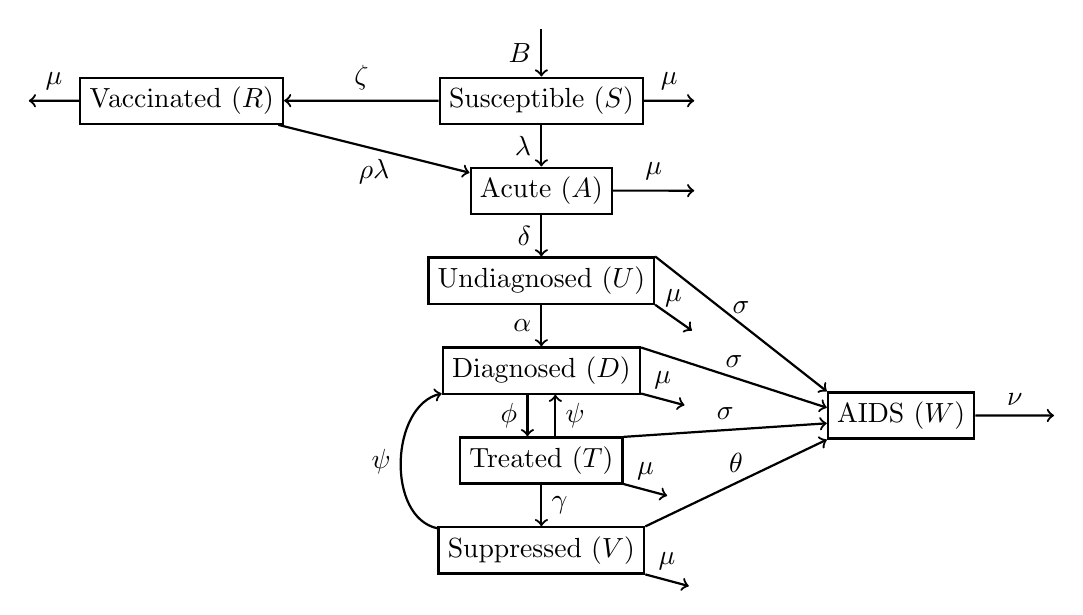
\begin{tikzpicture}[
  thick,
  scale = 1.142,
  compartment/.style = {draw},
  ]

  \node at (0, 5)
  [compartment, name = Susceptible] {Susceptible ($S$)};

  \node at (-4, 5)
  [compartment, name = Vaccinated] {Vaccinated ($R$)};

  \node at (0, 4)
  [compartment, name = Acute] {Acute ($A$)};

  \node at (0, 3)
  [compartment, name = Undiagnosed] {Undiagnosed ($U$)};

  \node at (0, 2)
  [compartment, name = Diagnosed] {Diagnosed ($D$)};

  \node at (0, 1)
  [compartment, name = Treated] {Treated ($T$)};

  \node at (0, 0)
  [compartment, name = Suppressed] {Suppressed ($V$)};

  \node at (4, 1.5)
  [compartment, name = AIDS] {AIDS ($W$)};

  \draw [->] (Susceptible) to node [left] {$\lambda$} (Acute);

  \draw [->] (Susceptible) to node [above] {$\zeta$} (Vaccinated);

  \draw [->] (Vaccinated) to node [below] {$\rho \lambda$} (Acute);

  \draw [->] (Acute) to node [left] {$\delta$} (Undiagnosed);

  \draw [->] (Undiagnosed) to node [left] {$\alpha$} (Diagnosed);

  \draw [->] (Diagnosed.240) to node [left] {$\phi$} (Treated.120);

  \draw [->] (Treated.60) to node [right] {$\psi$} (Diagnosed.300);

  \draw [->] (Treated) to node [right] {$\gamma$} (Suppressed);

  \draw [->] (Suppressed) to [out = 168, in = 193] node [left] {$\psi$} (Diagnosed);

  \draw [->] (Undiagnosed.12) to node [above] {$\sigma$} (AIDS.162);

  \draw [->] (Diagnosed.13) to node [above] {$\sigma$} (AIDS.174);

  \draw [->] (Treated.16) to node [above] {$\sigma$} (AIDS.186);

  \draw [->] (Suppressed.13) to node [above] {$\theta$} (AIDS.198);

  \draw [<-] (Susceptible) to node [left] {$B$} +(90: 0.8);

  \draw [->] (Susceptible) to node [above] {$\mu$} +(0: 1.7);

  \draw [->] (Vaccinated) to node [above] {$\mu$} +(0: -1.7);

  \draw [->] (Acute) to node [above] {$\mu$} +(0: 1.7);

  \draw [->] (Undiagnosed.348) to node [above] {$\mu$} +(325: 0.5);

  \draw [->] (Diagnosed.347) to node [above] {$\mu$} +(345: 0.5);

  \draw [->] (Treated.344) to node [above] {$\mu$} +(345: 0.5);

  \draw [->] (Suppressed.347) to node [above] {$\mu$} +(345: 0.5);

  \draw [->] (AIDS) to node [above] {$\nu$} +(0: 1.7);

\end{tikzpicture}


%%% Local Variables:
%%% mode: latex
%%% TeX-master: "model"
%%% End:

  \caption{Model diagram.}
\end{figure}


\begin{equation}
  \label{model_eqns}
  \begin{split}
    \frac{\md S}{\md t} &= B N - \lambda S - \zeta S- \mu S,
    \\
     \frac{\md R}{\md t} & = \zeta S - \rho \lambda R - \mu R,
    \\
    \frac{\md A}{\md t} &= \lambda S +\rho \lambda R - \delta A - \mu A,
    \\
    \frac{\md U}{\md t} &= \delta A - \alpha U - \mu U - \sigma U,
    \\
    \frac{\md D}{\md t} &=  \alpha U + \psi T + \psi V
    - \phi D - \mu D - \sigma D,
    \\
    \frac{\md T}{\md t} &= \phi D - \psi T - \gamma T - \mu T
    - \sigma T,
    \\
    \frac{\md V}{\md t} &= \gamma T - \psi V - \mu V - \theta V,
    \\
    \frac{\md W}{\md t} &= \sigma U + \sigma D + \sigma T + \theta V -
    \nu W,
  \end{split}
\end{equation}
with
\begin{equation}
  \label{force_of_infection}
  \begin{split}
    \lambda &= \frac{\beta_A A + \beta_U (U + D + T) + \beta_T V}{N},
    \\
    N &= S + R +  A + U + D + T + V,
    \\
    \beta_x &= c \left[1 - (1 - \tau_x)^n\right]
    \text{ for $x \in \{A, U, T\}$},
    \\
    \tau_T &= (1 - \epsilon) \tau_U.
  \end{split}
\end{equation}

The proportion diagnosed is
\begin{equation}
  p_D = \frac{D + T + V + W}{A + U + D + T + V + W},
\end{equation}
the proportion treated is
\begin{equation}
  p_T = \frac{T + V + W}{D + T + V + W},
\end{equation}
and the proportion with viral suppression is
\begin{equation}
  p_V = \frac{V}{T + V + W}.
\end{equation}

The targets for the proportions $p_D$, $p_T$, and $p_V$ are all:
if the initial level $p_x(0)$ is less than $90\%$, it will increase
linearly in the first 5 years and then stay at $90\%$ for the
remaining time; and if the initial level is at $90\%$ or above, it
will stay constant for the whole time:
\begin{equation}
  p_x^*(t)
  = p_x(0) + \left[
    \max\left\{0.9, p_x(0)\right\} - p_x(0)
  \right]
  \min\left\{\frac{t}{5}, 1\right\},
\end{equation}
for $x \in \{D, T, V\}$.


Similarly, the proportion of people vaccinated is
\begin{equation}
P_{V} = \frac{R}{S+R},
\end{equation}

We can implement it in the same way as the other controls. When we begin
vaccination in 2020/2025 the initial vaccination level is 0\%, the it
will increase linearly in the first year and then stay at 50\% for the
remaining time.
\begin{equation}
P^{*}_{V}(t) =
  \begin{cases}
    0 & \text{if $t < 5$ or $10$},
    \\
    0.5  & \text{if $t \geq 5$ or $10$},
  \end{cases}
\end{equation}


\section{Rates that are on when $p_x < p^*_x$}

The rates turn on when the proportions are below the target levels:
\begin{equation}
  \begin{split}
    \alpha(t) &= \alpha_{\max} H\left(p_D^*(t) - p_D(t)\right),
    \\
    \phi(t) &= \phi_{\max} H\left(p_T^*(t) - p_T(t)\right),
    \\
    \psi(t) &= \psi_{\max} H\left(p_V(t) - p_V^*(t)\right),
    \\
    \zeta(t) &= \zeta_{max} H\left(P^{*}_{V}(t)-P_{V}(t)\right),
  \end{split}
\end{equation}
where $H(x)$ is the Heaviside function
\begin{equation}
  H(x) =
  \begin{cases}
    0 & \text{if $x < 0$},
    \\
    1 & \text{if $x > 0$}.
  \end{cases}
\end{equation}

The discontinuity of the Heaviside function makes numerical solution
difficult.  Instead, replace $H$ with the continuous piecewise linear
function
\begin{equation}
  H(x) =
  \begin{cases}
    0 & \text{if $x < 0$},
    \\
    x / \chi & \text{if $0 \leq x \leq \chi$},
    \\
    1 & \text{if $x > \chi$},
  \end{cases}
\end{equation}
with some small value of $\chi$.


\section{$R_0$}

The infected states are
\begin{equation}
  \vec{x} = \left(A, U, D, T, V, W\right)^{\mT}.
\end{equation}
The flow for the infected states is
\begin{equation}
  \frac{\md \vec{x}}{\md t} =
  \begin{pmatrix}
    \lambda (S +\rho R) - (\delta + \mu) A
    \\
    \delta A - (\alpha + \mu + \sigma) U
    \\
    \alpha U + \psi T + \psi V - (\phi + \mu + \sigma) D
    \\
    \phi D - (\psi + \gamma + \mu + \sigma) T
    \\
    \gamma T - (\psi + \mu + \theta) V
    \\
    \sigma U + \sigma D + \sigma T + \theta V - \nu W
  \end{pmatrix}
\end{equation}
with
\begin{align}
  \lambda &= \frac{\beta_A A + \beta_U (U + D + T) + \beta_T V}{N},
  &
  N &= S + R + A + U + D + T + V.
\end{align}
The rate of new infections and transitions are
\begin{align}
  \mathcal{F}(\vec{x}) &=
  \begin{pmatrix}
    \lambda (S +\rho R)
    \\
    0
    \\
    0
    \\
    0
    \\
    0
    \\
    0
  \end{pmatrix},
  &
  \mathcal{V}(\vec{x}) &=
  \begin{pmatrix}
    (\delta + \mu) A
    \\
    - \delta A + (\alpha + \mu + \sigma) U
    \\
    - \alpha U - \psi T - \psi V + (\phi + \mu + \sigma) D
    \\
    - \phi D + (\psi + \gamma + \mu + \sigma) T
    \\
    - \gamma T + (\psi + \mu + \theta) V
    \\
    - \sigma U - \sigma D - \sigma T - \theta V + \nu W
  \end{pmatrix}.
\end{align}
The linearizations at $\vec{x}_0$ are
\begin{equation}
  \mat{F}
  =
  \begin{bmatrix}
    \beta_A z_0
    &
    \beta_U z_0
    &
    \beta_U z_0
    &
    \beta_U z_0
    &
    \beta_T z_0
    &
    0
    \\
    0 & 0 & 0 & 0 & 0 & 0
    \\
    0 & 0 & 0 & 0 & 0 & 0
    \\
    0 & 0 & 0 & 0 & 0 & 0
    \\
    0 & 0 & 0 & 0 & 0 & 0
    \\
    0 & 0 & 0 & 0 & 0 & 0
  \end{bmatrix}
\end{equation}
and
\begin{equation}
  \mat{V} =
  \begin{bmatrix}
    \delta + \mu & 0 & 0 & 0 & 0 & 0
    \\
    - \delta & \alpha + \mu + \sigma & 0 & 0 & 0 & 0
    \\
    0 & - \alpha & \phi + \mu + \sigma & - \psi & - \psi & 0
    \\
    0 & 0 & - \phi & \psi + \gamma + \mu + \sigma & 0 & 0
    \\
    0 & 0 & 0 & - \gamma & \psi + \mu + \theta & 0
    \\
    0 & - \sigma & - \sigma & - \sigma & - \theta & \nu
  \end{bmatrix},
\end{equation}
with
\begin{equation}
  z_0 = \frac{S_0 + \rho R_0}{S_0 + R_0}
  = (1 - v) + \rho v,
\end{equation}
where $v$ is vaccine coverage.

If $\alpha = \phi = \psi = 0$, then $D = T = V = 0$ for all time, so
we can drop them:
\begin{align}
  \mat{F}
  &=
  \begin{bmatrix}
    \beta_A z_0 & \beta_U z_0 & 0
    \\
    0 & 0 & 0
    \\
    0 & 0 & 0
  \end{bmatrix}
  &
  \mat{V} &=
  \begin{bmatrix}
    \delta + \mu & 0 & 0
    \\
    - \delta & \mu + \sigma & 0
    \\
    0 & - \sigma & \nu
  \end{bmatrix},
\end{align}

The residence times are $\mat{V}^{-1}$, which in the reduced case is
\begin{equation}
  \mat{V}^{-1} =
  \begin{bmatrix}
    \frac{1}{\delta + \mu} & 0 & 0
    \\
    \frac{\delta}{\delta + \mu} \frac{1}{\mu + \sigma}
    & \frac{1}{\mu + \sigma} & 0
    \\
    \frac{\delta}{\delta + \mu} \frac{\sigma}{\mu + \sigma}
    \frac{1}{\nu}
    & \frac{\sigma}{\mu + \sigma} \frac{1}{\nu} &\frac{1}{\nu}
  \end{bmatrix}.
\end{equation}

The next-generation matrix is $\mat{G} = \mat{F} \mat{V}^{-1}$, which
in the reduced case is
\begin{equation}
  \mat{G} =
  \begin{bmatrix}
    \left(\beta_A \frac{1}{\delta + \mu}
      + \beta_U \frac{\delta}{\delta + \mu}
      \frac{1}{\mu + \sigma}\right)
    z_0
    & 
    \beta_U \frac{1}{\mu + \sigma} z_0
    &
    0
    \\
    0 & 0 & 0
    \\
    0 & 0 & 0
  \end{bmatrix}.
\end{equation}
This has eigenvalues
\begin{equation}
  \left\{\left(\beta_A \frac{1}{\delta + \mu}
      + \beta_U \frac{\delta}{\delta + \mu}
      \frac{1}{\mu + \sigma}\right)
    z_0, 0, 0
  \right\},
\end{equation}
the largest of which is $R_0$:
\begin{equation}
  R_0 = \left(\beta_A \frac{1}{\delta + \mu}
    + \beta_U \frac{\delta}{\delta + \mu}
    \frac{1}{\mu + \sigma}\right)
  z_0.
\end{equation}

\end{document}
